\documentclass[main.tex]{subfiles} % Subfile-Class



% ============================================================================== %
%                            Subfile document                                    %
% ============================================================================== %

\begin{document}

% Template

\subsubsection{Liniensensor}

Im folgenden Abschnitt ist die Entwicklung und Evaluierung eines Liniensensors
dokumentiert. Ziel ist es, einen einfach auszuwertenden Sensor zu entwickeln,
der das vorgegebene Klebeband (\textit{Tesa Gewebeband 4651}) problemlos vom Wettkampf-Untergrund unterscheiden kann.\\
Ein eigener Liniensensor wird entwickelt, weil das Verlassen der Strecke als ein hohes Risiko empfunden wird. Daher ermöglicht
das eigene Designen eines Liniensensors eine hohe flexibilität. Dies mit der Begründung, dass für ein massgeschneidertes Produkt 
alle Komponenten selber erlesen werden können.


% ===================================================================================
\subsubsection*{Anforderungen}

Das Klebeband muss auf einem rötlich
gefliesten Untergrund detektiert werden. Eine besondere Herausforderung
stellen hierbei längs und querverlaufende Fliesenfugen dar, welche eine
ähnliche Farbe aufweisen. Dieser Untergrund ist in
Abbildung~\ref{fig:Untergrund_Wettkampf} gezeigt.

\begin{figure}[H]
    \centering
    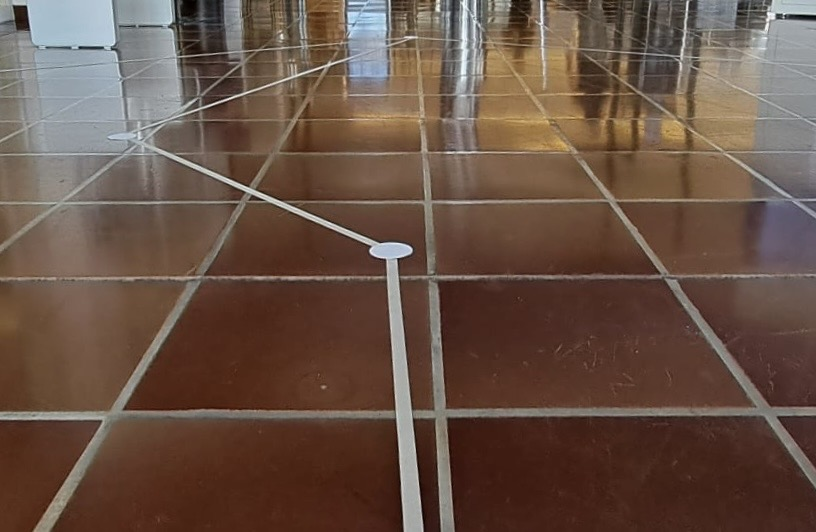
\includegraphics[width=0.75\textwidth]{fig_Strecke_Tracken/Bild_Untergrund.jpg}
    \caption{Untergrund während des Wettkampfs}~\label{fig:Untergrund_Wettkampf}
\end{figure}

% ===================================================================================

\subsubsection*{Aufbau und Auswertung}
Der Liniensensor wird aus acht einzelnen Messzellen aufgebaut. Es werden acht Messzellen
gewählt, damit eine möglichst breite Fläche durch den Sensor abgedeckt werden kann, aber
dennoch nicht zu viele Pins für die Auswertung benötigt werden. Dabei sollten stets genau
zwei Messzellen direkt über dem Klebeband ausgerichtet sein. Jede einzelne Messzelle hat 
eine emittierende Diode und einen dazugehörigen Fototransistor. Je mehr Licht auf den 
Fototransistor einwirkt, desto höher ist der Strom, welcher durch ihn fliesst. Weil der 
Fototransistor als konstante Stromquelle interpretiert werden kann, wird der Spannungsabfall
über ihn ausgewertet. Ein hoher Strom durch den Fototransistor bewirkt einen hohen 
Spannungsverlust an einem davor geschaltenen Widerstand. Somit sollte die Spannung über dem
Fototransistor gegen Ground gezogen werden. Ist der Strom jedoch klein,
so fällt gemäss dem Ohmschen Gesetz wenig Spannung über dem Vorwiderstand ab was einen erhöhten
Spannungsabfall über dem Fototransistor zur Folge hat. Diese Spannungen werden dann mittels
Analog-Digital-Wandlern (ADCs) ausgewertet. In Abbildung~\ref{fig:Auswertung_Liniensensor1} ist 
die Auswertung schematisch festgehalten.

\begin{figure}[H]
    \centering
    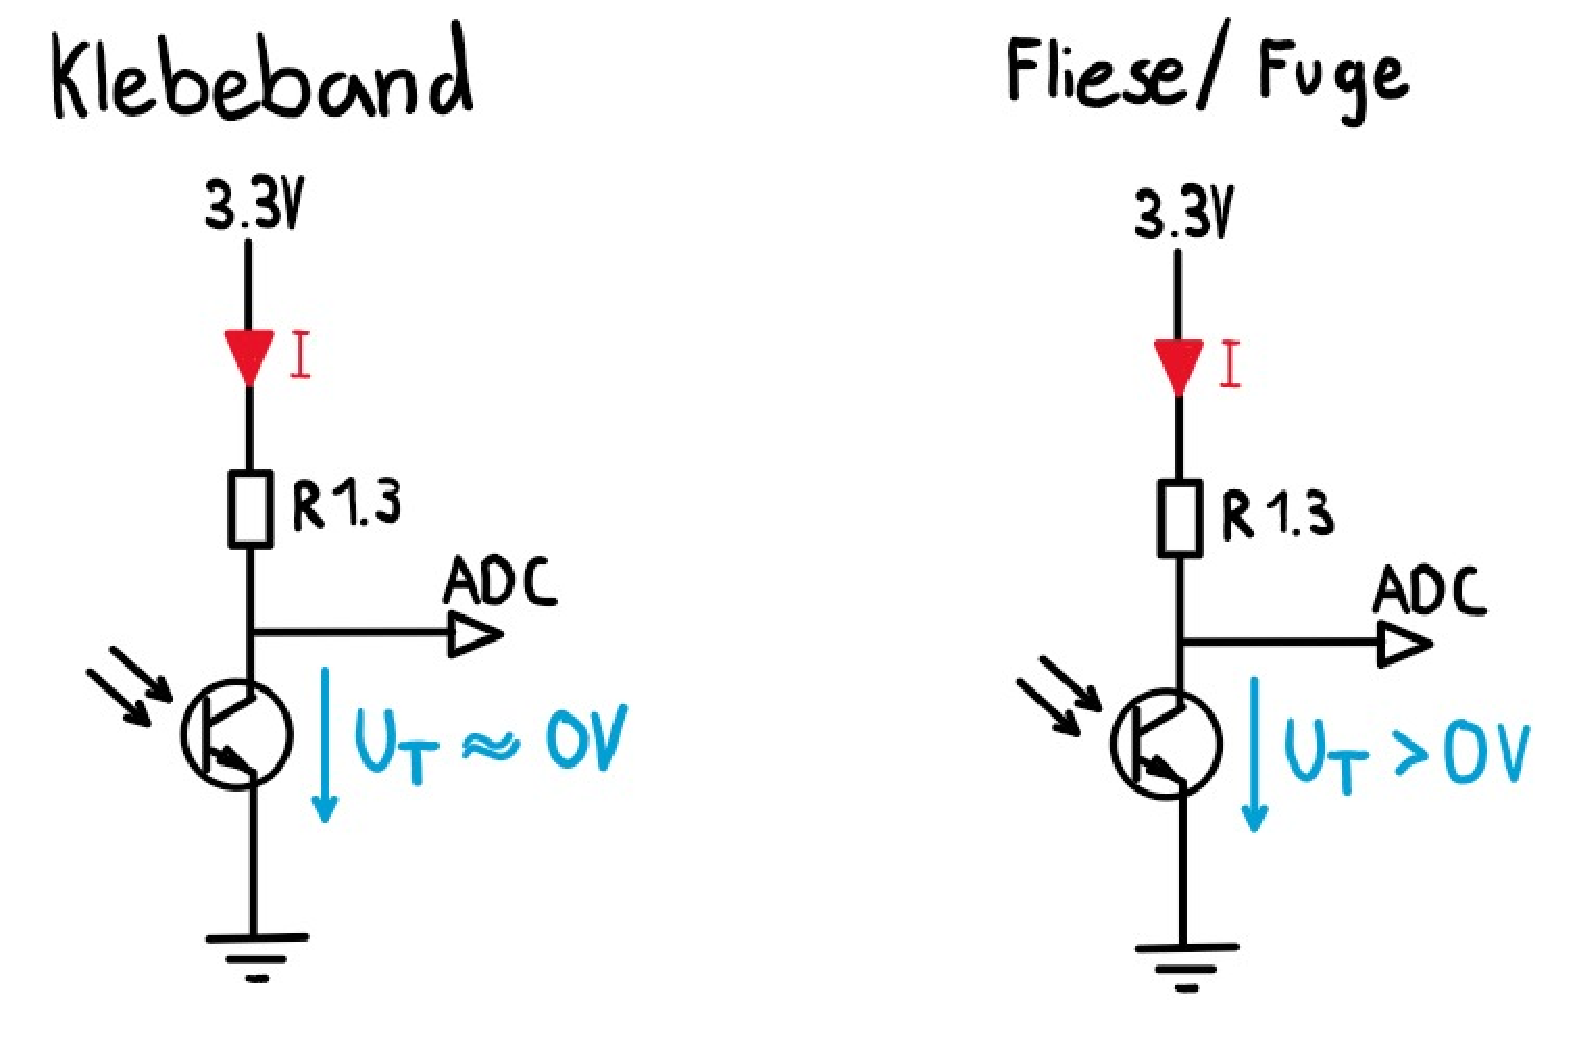
\includegraphics[width=0.5\textwidth]{fig_Strecke_Tracken/Auswertung_Liniensensor.pdf}
    \caption{Konzept der Auswertung mittels ADC}~\label{fig:Auswertung_Liniensensor1}
\end{figure}


% ===================================================================================




\subsubsection{Liniensensor als PCB}

Damit der Liniensensor möglichst praxisnah getestet 
werden kann, wird dieser als PCB mit Kicad erstellt. Dabei werden die 
oben formulierten Anforderungen und Dimensionierungen eingehalten. In Abbildung~\ref{fig:Liniensensor_Top} 
ist die Draufsicht und in Abbildung~\ref{fig:Liniensensor_Bottom} die Untersicht dargestellt.

\begin{figure}[H]
    \centering
    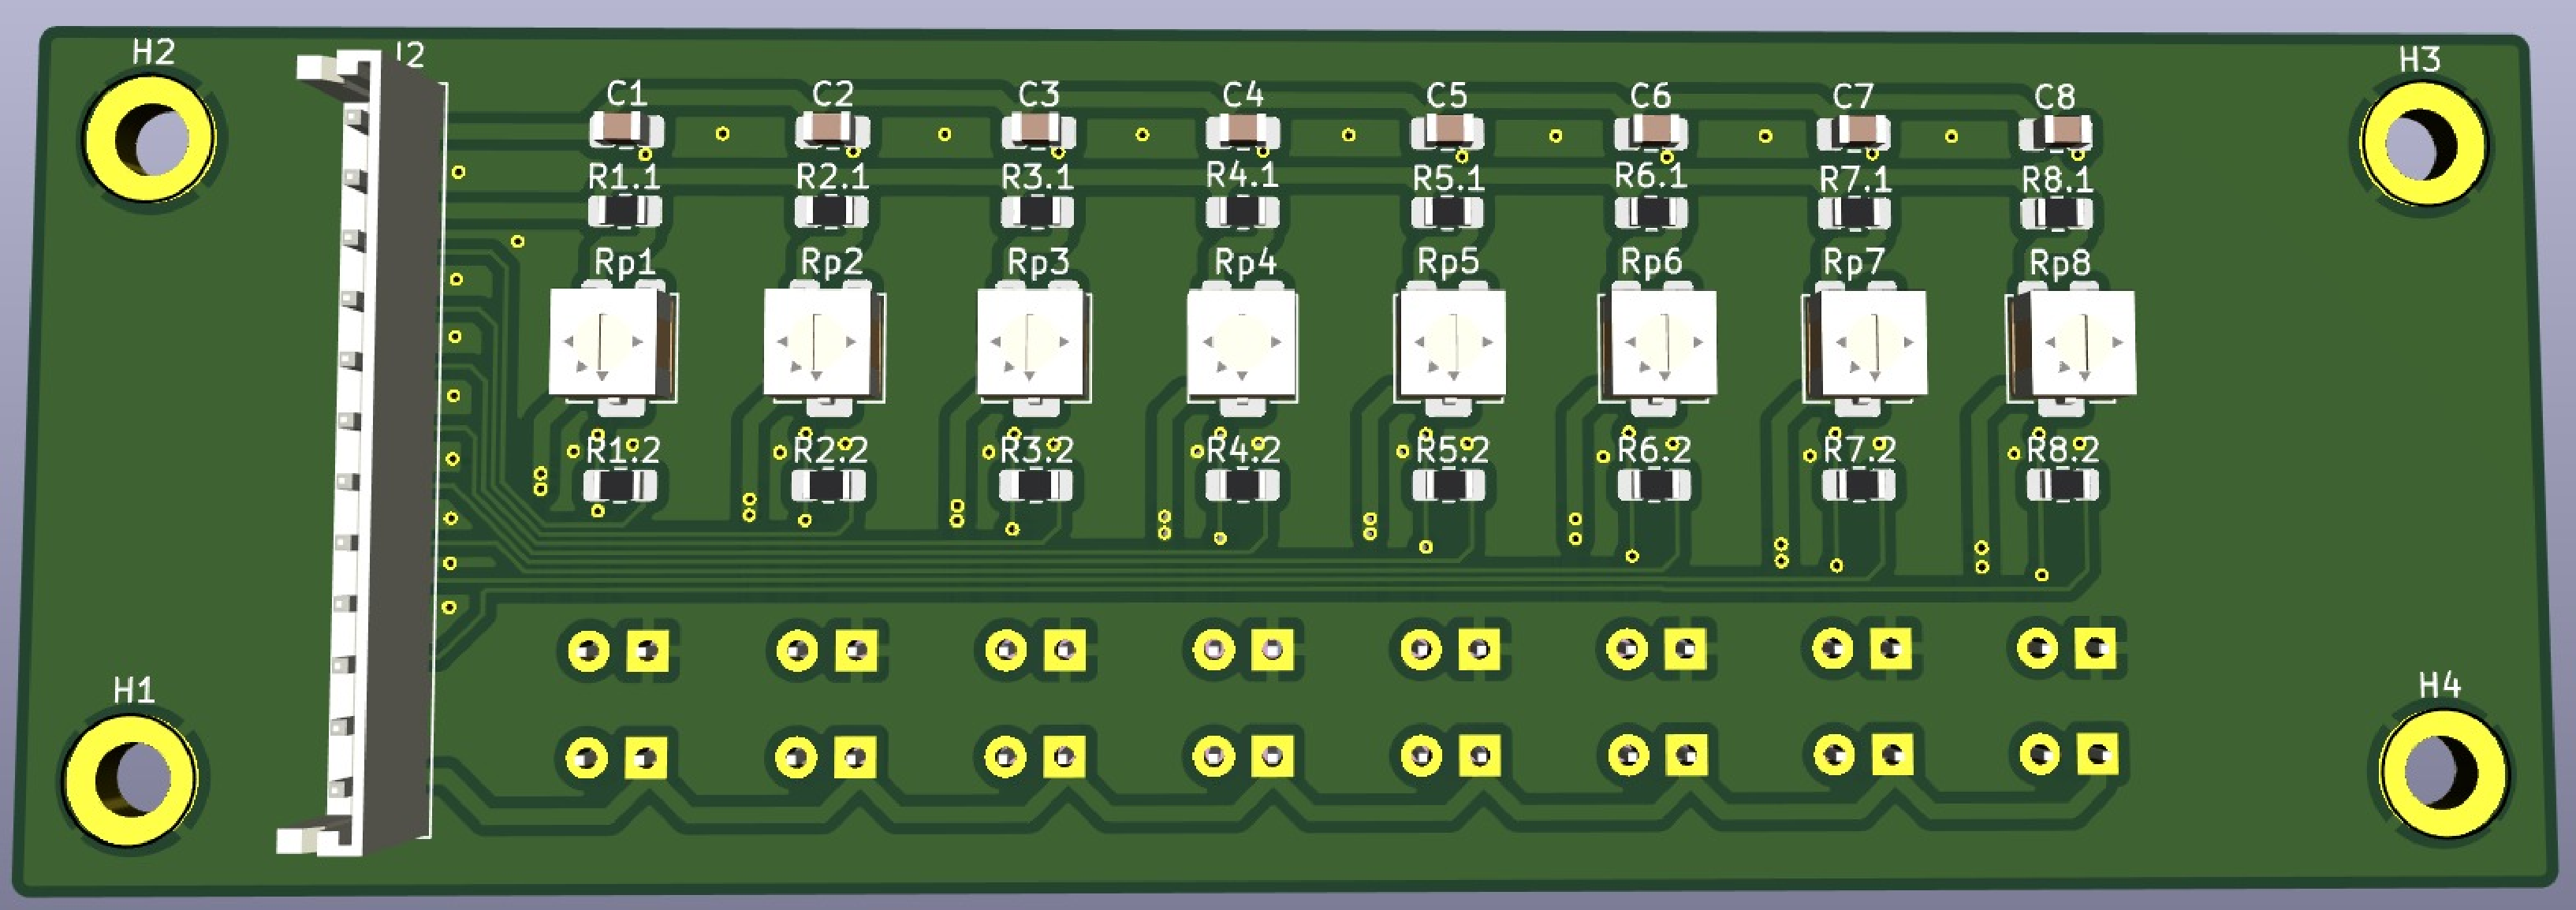
\includegraphics[width=0.75\textwidth]{fig_Strecke_Tracken/Liniensensor_Top.pdf}
    \caption{Liniensensor in Kicad von oben}~\label{fig:Liniensensor_Top}
\end{figure}

\begin{figure}[H]
    \centering
    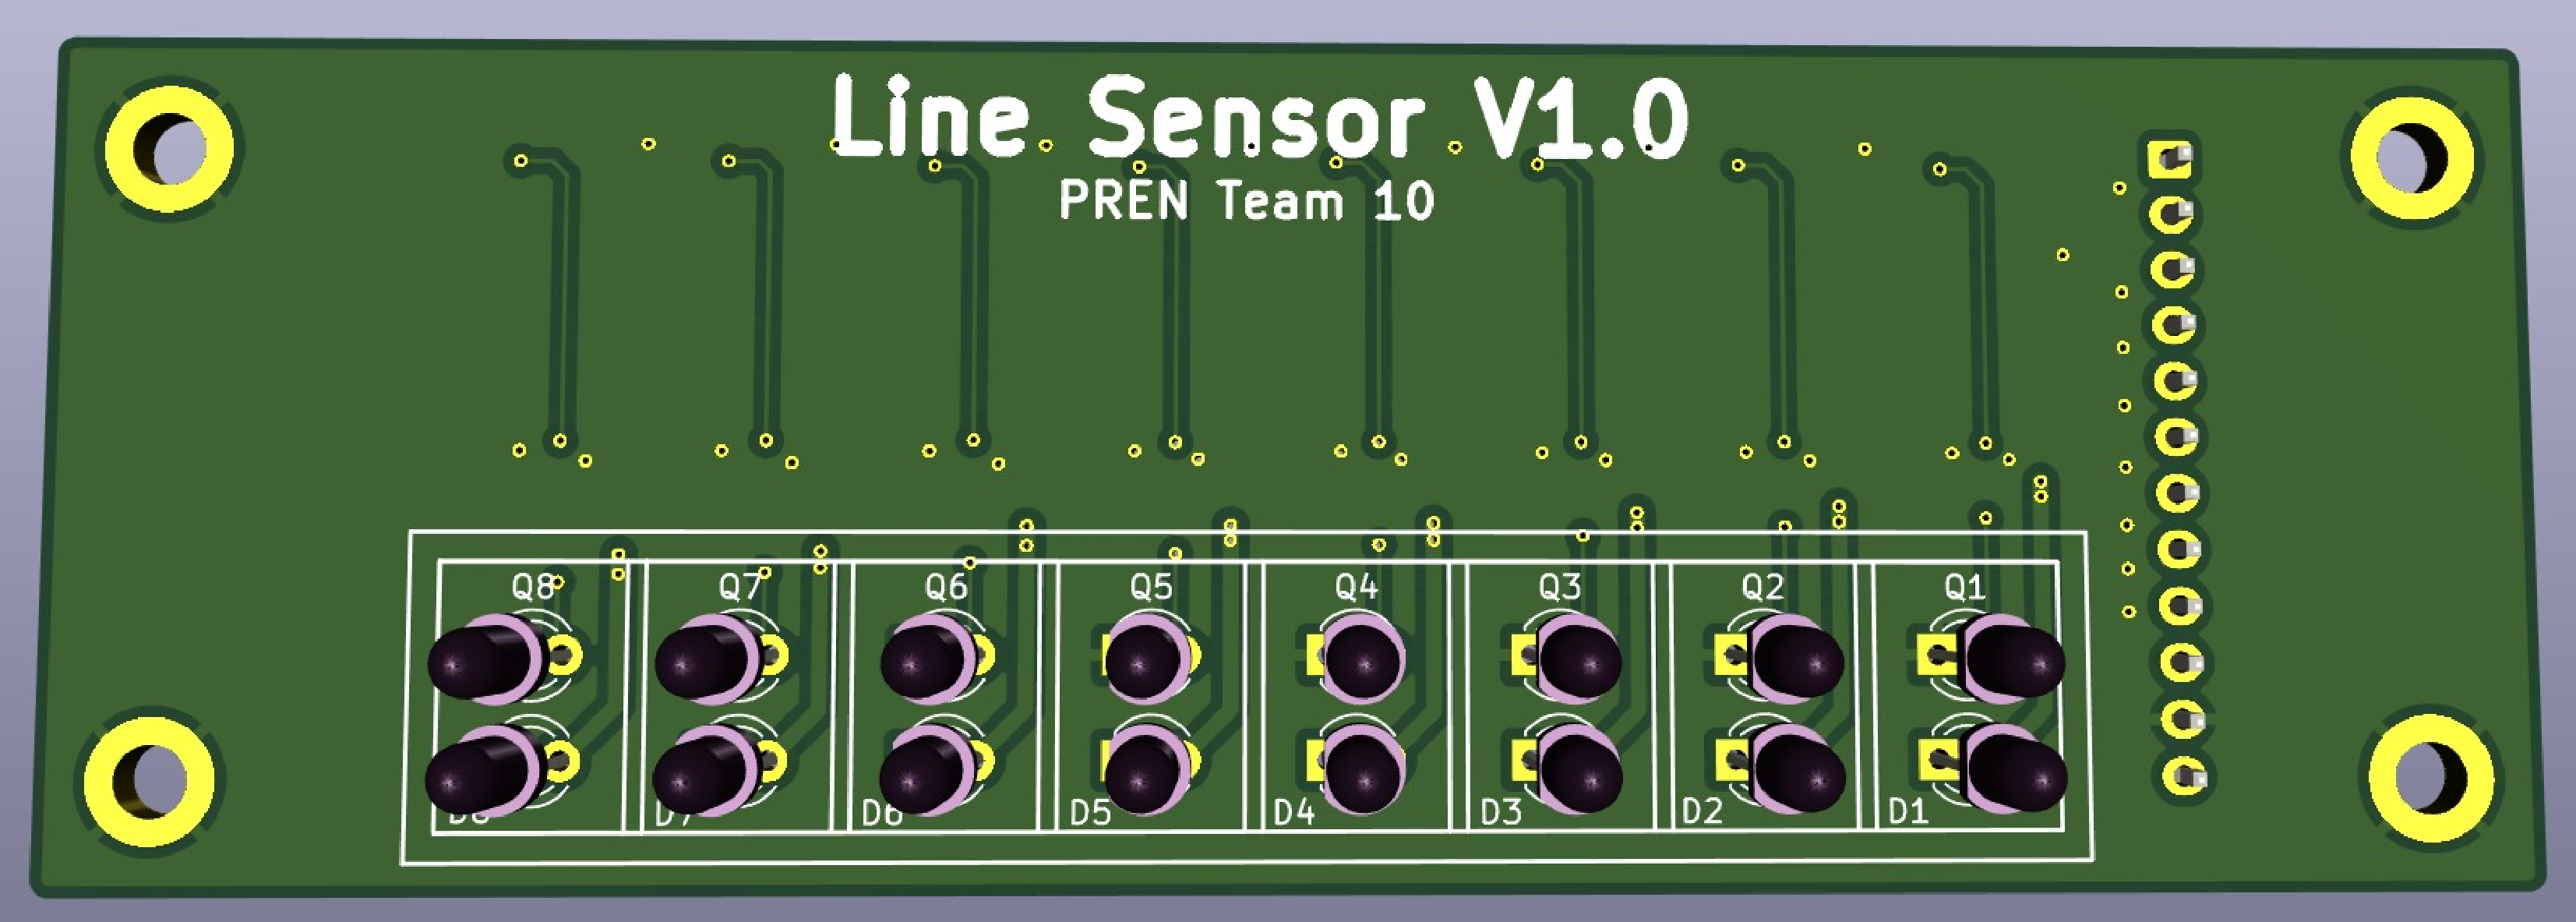
\includegraphics[width=0.75\textwidth]{fig_Strecke_Tracken/Liniensensor_Bottom.pdf}
    \caption{Liniensensor in Kicad von unten}~\label{fig:Liniensensor_Bottom}
\end{figure}




% ===================================================================================

\paragraph{Versuche}
Im Anhang ist ein Versuch dokumentiert, welcher ein geeignetes Lichtspektrum für den Liniensensor liefert. Ausserdem wurden
die Ströme auf den unterschiedlichen Untergründen (Klebeband, Fliese und Fuge) gemessen. Mittels eines 
Arduino wurden alle Eingänge ausgewertet und der Liniensensor validiert. 
Alle Messungen sind im Anhang~\ref{anhang:Liniensensor} dokumentiert.

% ===================================================================================
\paragraph{Entscheidung und Fazit}
Durch die Messungen wurde das 
Konzept des Liniensensors überprüft und validiert. Das folgende Bild bestätigt, dass das Klebeband
von der Fliese deutlich unterschieden werden kann. Die Abbildung~\ref{fig:Auswertung_Strecke_Beispiel} zeigt
die Spannungsauswertung mittels ADCs. Diese Auswertung wurde mit einem Arduino gemacht. Die hohen 
Werte stellen die Fliese dar und die tiefen Werte das Klebeband.

\begin{figure}[H]
    \centering
    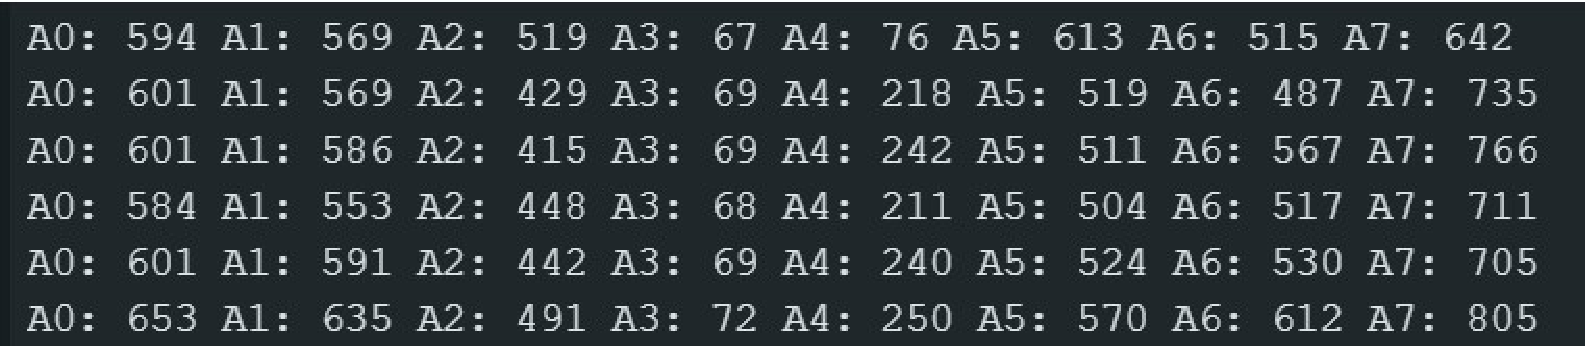
\includegraphics[width=0.75\textwidth]{fig_Strecke_Tracken/Auswertung_Strecke.pdf}
    \caption{Die tiefen Werte stellen das Klebeband dar und die hohen die Fliesen}~\label{fig:Auswertung_Strecke_Beispiel}
\end{figure}

Auf der Abbildung ist ersichtlich, dass sich A3 direkt überhalb dem Klebeband befindet. Die Pins A2 und A4 sind 
teilweise auch über dem Klebeband. Der Wert ist allerdings grösser, weil nur ein Teil des Klebebandes direkt darunter
liegt.\\
Anfangs wurde der Unterschied von Klebeband zu Fugen als eine Schwierigkeit betrachtet. Der Lininensensor ist fähig, 
Fugen von Klebeband zu unterscheiden. Dies ist im Anhang~\ref{anhang:Liniensensor} genauer dokumentiert.\\
Aufgrund der eindeutigen Messwerten, wird dieser Liniensensor verwendet.


\end{document}
